\section{Introduction}











\section{\#SAT}




%
%\begin{frame}{Why Quantum Computing?}
%
%\centering
%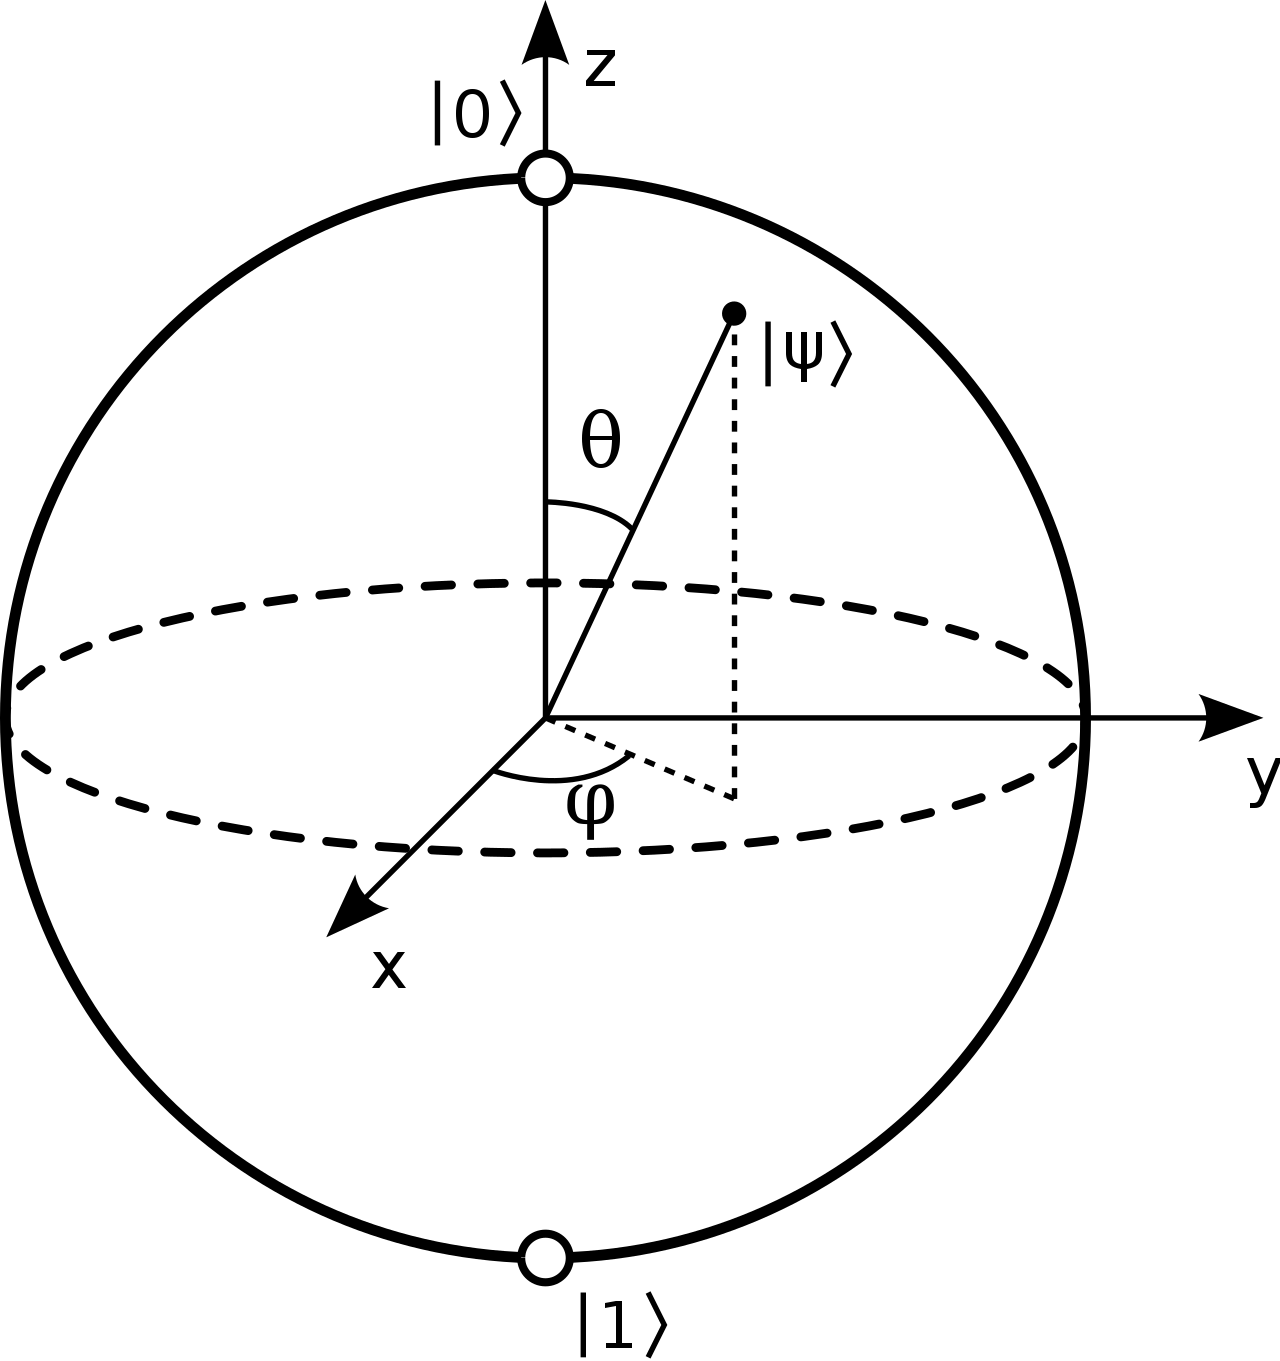
\includegraphics[width=2.5cm]{Bloch_sphere.svg.png}
%
%
%	\begin{block}{\bf A few reasons ..}
%		\begin{itemize}
%		\item Some evidence that quantum can solve classically intractable problems
%  		\item Nature is inherently quantum
%		\begin{itemize}
%  		\item Physicists and chemists need to solve hard simulation problems
%  		\item Many problems physicists deal with are \QMA-complete (``Quantum \NP'')
%		\end{itemize}
%		\item Classical hardware is reaching its limitations
%		\begin{itemize}
%  		\item Quantum effects, like tunneling, put a spoke in the wheel
%%  		\item Philosophically interesting
%		\end{itemize}
%		\end{itemize}
%	\end{block}
%
%\end{frame}
%

%\begin{frame}{Why NOT Quantum Computing?}
%\begin{refsection}
%
%\vfill
%
%\begin{alertblock}{What if the (error-corrected) quantum computer never materializes?}
%		\begin{itemize}
%		\item it turns out that \BQP{} = \P, or
%		\item the device is too hard to build
%		\end{itemize}
%\end{alertblock}
%
%\centering
%
%
%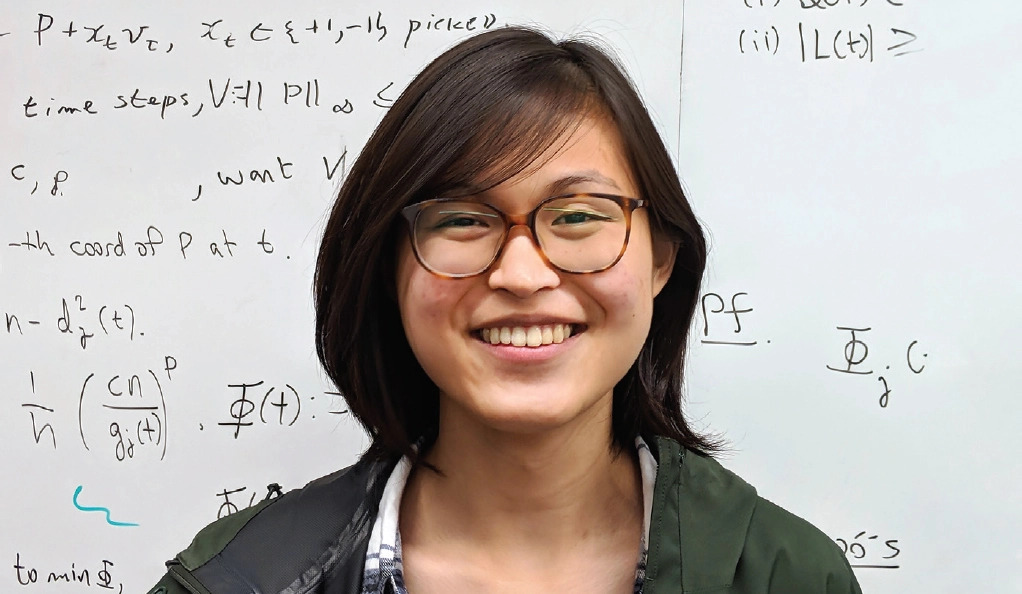
\includegraphics[width=4cm]{tang.jpeg}
%
% Ewin Tang~\cite{tang2019quantum}
%
%\onslide<2->{
%\alert{Regardless of whether a quantum computer ever gets build, we are improving our understanding of quantum-hard problems.}
%}
%
%%\vspace{-.5em}
%
%\vfill
%\printbibliography[section=\therefsection]
%
%\end{refsection}
%\end{frame}




%\begin{frame}{On the Road to Quantum Supremacy}
%
%
%\[
%\scalebox{.8}{
%\Qcircuit @C=1.em @R=.7em {
%\lstick{\ket{0}} & & \gate{H} & \ctrl{1} 						&\qw	& \qw      & \qw  \\
%\lstick{\ket{0}} & & \qw      & \gate{X} 						&\qw 	& \ctrl{1} & \qw  \\
%\lstick{\ket{0}} &  & \qw      & \push{\rule{1.5em}{.4pt}}\qw 	& \qw 	& \gate{X} & \qw  
%}}
%\]
%
%~\\
%
%	\begin{block}{\bf How can we contribute?}
%		\begin{itemize}
%		\item Build an (error-corrected) quantum computer
%		\item Come up with a new quantum algorithm that (conditionally) shows that $\BQP \neq P$
%		\item {Invent the tools to use current and future quantum computers}
%\pause
%		\begin{itemize}
%		\item \alert{Comparing data structures for representing quantum information}
%		\item \alert{Quantum circuit compilation}
%		\item \alert{Simulation and analysis of physical systems}
%		\item \dots
%		\end{itemize}
%		\end{itemize}
%	\end{block}
%
%\end{frame}
%
%\begin{refsection}
%\begin{frame}{Quantum Circuit Compilation}
%
%
%	\begin{block}{\bf Compilation is essential}
%		\begin{itemize}
%		\item Efficiently utilize early frugile quantum computers
%%		\item ....
%		\item Error correction requires hybrid solutions with fast classical components
%		\end{itemize}
%	\end{block}
%
%\pause
%\vspace{-.5em}
%
%	\begin{block}{\bf Compilation entails...}
%		\begin{itemize}
%		\item {Quantum circuit simulation}~\cite{burgholzer2020advanced,viamontes2003improving,vinkhuijzen2021limdd}
%		\item Quantum circuit optimization (topology, gate type minimization, ...)~\cite{shaik2023optimal}
%%		\item Quantum circuit verification~\cite{}
%		\item Quantum circuit equivalence checking~\cite{thanos2023fast,peham2022equivalence}
%		\item Quantum circuit synthesis~\cite{brand2023quantum,}
%		\end{itemize}
%	\end{block}
%
%\vspace{-.8em}
%
%\printbibliography[section=\therefsection]
%
%\pause
%\centering
%\alert{(We can use the power of formal methods \& automated reasoning tools)}
%
%
%\end{frame}
%\end{refsection}




%
%\begin{frame}{Quantum Circuit Simulation}
%
%\vfill
%
%~~~~~~~~~~~~~~
%\Qcircuit @C=2.3em @R=0.7em {
%& \ket{0} & & \gate{H} & \ctrl{1} & \qw      & \qw  \\
%& \ket{0} & & \qw      & \gate{X} & \ctrl{1} & \qw \\
%& \ket{0} & & \qw      & \push{\rule{1.5em}{.4pt}}\qw & \gate{X} & \meter\\
%&	  & & \dstick{U_1} & \dstick{U_2} & \dstick{U_3}  	 & \dstick{U_4}
%\gategroup{1}{4}{3}{4}{.7em}{--}
%\gategroup{1}{5}{3}{5}{.7em}{--}
%\gategroup{1}{6}{3}{6}{.7em}{--}
%\gategroup{1}{7}{3}{7}{.7em}{--}
%}
%
%\vfill
%
%\vspace{1em}
%
%\pause
%\begin{exampleblock}{State-based simulation}
%\centering
%\scalebox{1.5}{
%$ \ket{\phi_1} ~~=~~ U_1 \cdot \ket{\phi_0} $
%}
%
%\scalebox{1.5}{
%$ \ket{\phi_2} ~~=~~ U_2 \cdot \ket{\phi_1} $
%}
%
%\scalebox{1.5}{
%$ \ket{\phi_3} ~~=~~ U_3 \cdot \ket{\phi_2} $
%}
%
%\scalebox{1.5}{
%$ \ket{\phi_4} ~~=~~ \hspace{-.07cm}\underbrace{U_4}_{\mathclap{\text{simple matrices}}}  \hspace{-.1cm} \cdot \ket{\phi_3} $
%}
%\end{exampleblock}
%
%\pause
%
%\begin{block}{Strong vs weak simulation}
%	\begin{itemize}
%		\item \textbf{Strong}: compute probability $\braket{b | \phi_3}$ of the measure outcome  for any $b\in \set{0,1}^n$
%		\item \textbf{Weak}: sample the probability distribution $b\in \set{0,1}^n \to \braket{b | \phi_3}$
%
%			\alert{(This is what a quantum computer does.)}
%	\end{itemize}
%\end{block}
%
%
%\vfill
%	
%\end{frame}
%


%\begin{refsection}
%\begin{frame}{Verification: Circuit Equivalence Checking}
%
%\vfill
%
%\centering
%
%
%\begin{columns}
%\begin{column}{.05\textwidth}
%\end{column}
%\begin{column}{.4\textwidth}
%\scalebox{1}{
%\Qcircuit @C=1.em @R=.7em {
%& & \gate{H} & \ctrl{1} 						&\qw	& \qw      & \qw  \\
%& & \qw      & \gate{X} 						&\qw 	& \ctrl{1} & \qw  \\
%&  & \qw      & \push{\rule{1.5em}{.4pt}}\qw 	& \qw 	& \gate{X} & \qw  
%}}
%\end{column}
%\begin{column}{.08\textwidth}
%\hspace{-.em}
%\scalebox{2}{$\stackrel?\approx$}
%\end{column}
%\begin{column}{.4\textwidth}
%\scalebox{1}{
%\Qcircuit @C=1em @R=.7em {
%& & \qw		  &  \gate{X}  						& \gate{H} 	& \qw      & \qw  \\
%& & \gate{H}  &  \ctrl{-1}\qwx[0] 				& \gate{H} 	& \ctrl{1} & \qw \\
%&  & \qw      & \push{\rule{1.5em}{.4pt}}\qw  	&\qw  		&   \gate{X}&\qw  
%}}
%\end{column}
%\begin{column}{.05\textwidth}
%\end{column}
%\end{columns}
%
%\vspace{.5cm}
%
%
%\pause
%
%
%We can reduce this problem to \alert{strong} simulation \cite{thanos2023fast}.
%
%(A reduction to weak simulation would imply ``Quantum \P'' = ``Quantum \NP'')
%
%
%\vfill
%
%\printbibliography[section=\therefsection]
%\end{frame}
%\end{refsection}





%\begin{frame}{Representing Quantum Information}
%%	\framesubtitle{The proof uses \textit{reductio ad absurdum}.}
%
%
%
%\begin{columns}%[onlywidth,T]
%	\begin{column}{1\textwidth}
%	\centering
%\[
%\def\arraystretch{1.15}
%\underbrace{\scalebox{2}{$\ket{\phi}$}}_{n \text{ qubit state}}
%~~~~~=~
%\left.
%\begin{bmatrix*}[c]
%    \frac{i+1}{\sqrt 6} \\ 0 \\ 0 \\ 0\\ \vdots \\0\\ \frac1{\sqrt 3} \\ 0 \\\frac1{\sqrt 3} 
%\end{bmatrix*}
%~~\right \}\text{$2^n$-sized vector}
%\]  
%	\end{column}
%\end{columns}
%
%\begin{alertblock}{The Problem}
%	\begin{itemize}
%		\item A quantum state on $n$ qubits has $2^n$ amplitudes (complex numbers)
%	\end{itemize}
%\end{alertblock}
%
%
%
%\end{frame}





\begin{frame}{This Talk}
	

\begin{block}{Quantum Computing with \#SAT}
	
	
	\begin{itemize}
		\item (Exact) Simulation of quantum circuits
		\item (Exact) Equivalence checking of quantum circuits
%		\item \dots
	\end{itemize}
	
\end{block}

\pause


\begin{block}{Data Structures for Quantum Information}
	\begin{itemize}
		\item {(Generalized) Stabilizer Formalism}
		\item {Decision Diagrams (DDs)}
%	\begin{itemize}
%		\item We introduce \alert{\limdd} to unify strengths of stabilizer formalism and DDs.
%	\end{itemize}
		\item Tensor Networks: Matrix Product State (MPS) in specific
%		\item Restrict Boltzmann Machine (RBM; a single layer neural network)
\pause
		\item Tradeoff: \alert{Succinctness} vs \alert{Tractability}

	\end{itemize}
	\vspace{-.5em}
\end{block}


\begin{columns}
\begin{column}{.45\textwidth}	
\centering
~~~~~~~~\begin{tikzpicture}\footnotesize
  \tikzset{venn circle/.style={circle,minimum width=2cm,fill=####1,opacity=0.4}}
  \node [venn circle=white,minimum width=4cm,draw] (A) at (0,0.3) {};
  \node  at (0,1.95) 			{State space};

  \node [venn circle = Red!40!white, ellipse,minimum height=2.2cm, minimum width=3.6cm] (L) at (0,0.6) {};
  \node  at (0,1.5) 		{poly-\alert{\limdd}};
  
  \node [venn circle = blue!70!white,text width=1.3cm,align=center,rotate=79,ellipse,minimum height=1.8cm, minimum width=2.5cm] (B) at (-.6,-.2) {};
  \node[text width=1.3cm,align=center]  at (-.7,-1.) {poly-MPS};


  \node [venn circle = green!70!white,text width=1.3cm,align=center,rotate=119,ellipse,minimum height=1.8cm, minimum width=2.5cm] (B) at (.6,-.2) {};
  \node[text width=1.3cm,align=center]  at (.9,-1.) {poly-RBM};



  \node [venn circle = Blue!100!white,text width=1cm,align=center, minimum width=1.cm] (B) at (-.5,.3) 	{\textcolor{white}{poly-QMDD}};						

  \node [venn circle = OliveGreen!100!white,text width=1cm,align=center, minimum width=1.cm] (C) at (.5,.2) {\textcolor{white}{Stabilizer states}};

\end{tikzpicture}
	\end{column}
	\begin{column}{.65\textwidth}
\setlength{\tabcolsep}{2pt}
\def\arraystretch{1.1}
\footnotesize
\begin{tabular}{|l@{\hspace{10pt}}|| *{5}{c|}| *{20}{c|}}
%\footnotesize
\hline
 & \multicolumn{5}{c||}{Queries} & \multicolumn{7}{c|}{Manipulation operations} \\
	& \rot{\samp} & \rot{\pro} & \rot{\eq}  & \rot{\inprod} & \multicolumn{1}{R{90}{0em}||}{\fid}
	& \rot{\addi} & \rot\had & \rot{\xyz} & \rot\cz & \rot{\swap} & \rot{\loc} & \rot{\T-gate} \\
\hline
Vector& \Yar & \Yes & \Yes & \Yes & \Yes & \Yes & \Yes & \Yes & \Yes & \Yes & \Yes & \Yes \\
\hline
%		| Sampl	| Prob 	| Eq	|Inprod	| Fid
ADD   	& \Yar	& \Yes	& \Yes	& \Yes & \Yes
%		| Add	| H		| XYZ	| CX	| Swap	| Local	| T
		& \Yes	& \Yes 	& \Yes	& \Yes	& \Yes	& \Yes	& \Yes \\
\hline
QMDD
		& \Yar	& \Yes	& \Yes	& \Yes & \Yes
		& \No	& \No 	& \Yes	& \Yes	& \No	& \No	& \Yes \\
\hline 
%QMDD  & \Yes & \Yes & \Yes & \No & \Yes & \No & ?? & ??  & ?? & \No & ?? & ??   \\
%\hline    
\alert{\limdd} 	& \Yar	& \Yes	& \Yes	& \Cond & \Cond
		& \No	& \No	& \Yes	& \Yes	& \No	& \No	& \Yes  \\
\hline 
%TN    & \Cond? & \Cond? & \Cond? & \Cond? & ?? & \Yes? & \Yes? & \Yes? & \Yes? & \Yes? & \Yes? \\ \hline
MPS   & \Yar & \Yes & \Yes & \Yes & \Yes & \Yes 
	  & \Yes & \Yes & \Yes & \Yes & \Yes & \Yes  \\
\hline 
RBM   & \Yar    & ? & ? & \Cond & \Cond & ? & ? & \Yes & \Yes & \Yes & ? & \Yes \\
\hline 
%\multicolumn{13}{c}{Low priority} \\
%\hline 
%ZX    & ?? & ?? & ?? & ?? & ?? & ?? & ?? & ?? & ?? & ?? & ?? & ?? \\
%\hline 
%SLDD$_+$  & \Yes? & \Yes? & \Yes? & \Yes? & \Yes? & \No! & \No? & \Yes? & \No! & \No! & \No? & \Yes! \\
%\hline 
\end{tabular}	
\end{column}
\end{columns}

\end{frame}

















%\begin{frame}
%\vfill
%
%
%\Large
%
%\begin{quote}
%``Quantum computing becomes easy once you take the physics out of it''
%\end{quote}
%\hfill
%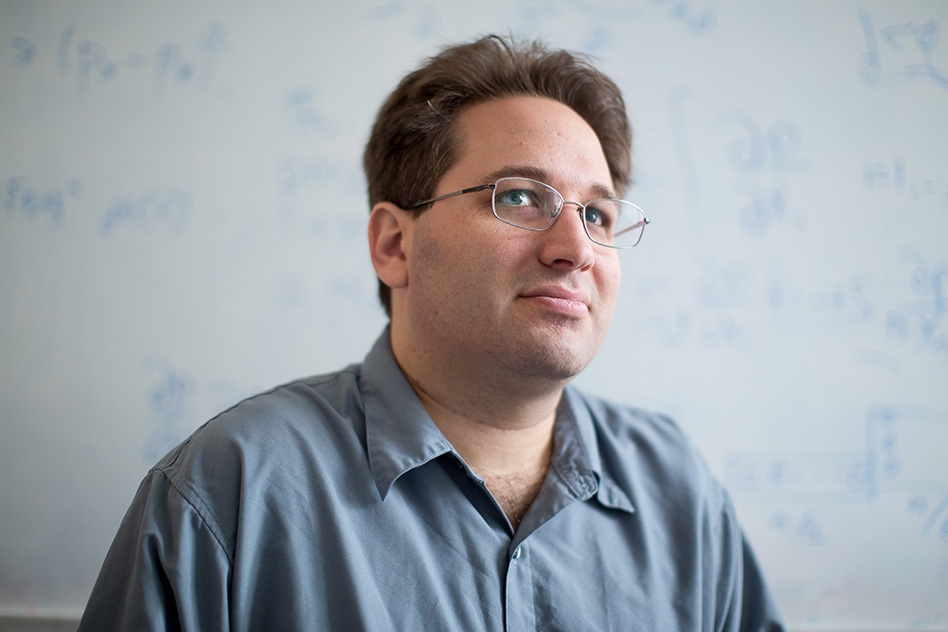
\includegraphics[width=5cm]{scott-aaronson.jpeg}
%
%\hfill Scott Aaronson
%
%%\hfill \url{https://scottaaronson.blog}
%\end{frame}
%
%
%
%
%
%
%
%
%\begin{frame}{Quantum States}
%%	\framesubtitle{The proof uses \textit{reductio ad absurdum}.}
%
%
%
%\begin{columns}%[onlywidth,T]
%	\begin{column}{.4\textwidth}
%\[
%\def\arraystretch{1.15}
%\underbrace{\scalebox{2}{$\ket{\phi}$}}_{n \text{ qubit state}}
%~~~~~=~
%\left.
%\begin{bmatrix*}[c]
%    \frac{i+1}{\sqrt 6} \\ 0 \\ 0 \\ 0\\ \vdots \\0\\ \frac1{\sqrt 3} \\ 0 \\\frac1{\sqrt 3} 
%\end{bmatrix*}
%~~\right \}\text{$2^n$-sized vector}
%\]  
%	\end{column}
%%\pause
%	\begin{column}{.6\textwidth}
%\vspace{3mm}\[
%\def\arraystretch{1.2}
%\scalebox{1.}{$\ket{00\dots01}$}
%~=~
%\begin{bmatrix*}[c]
%    0 \\ 1 \\ 0 \\ 0\\ \vdots \\0\\ 0  \\ 0 \\ 0 
%\end{bmatrix*}
%\begin{matrix*}[c]
%	{\text{$\leftarrow$ index \scriptsize 00\dots00 }} \\ 
%	{\text{$\leftarrow$ index \scriptsize 00\dots01 }} \\ \\ \\ \\ \\ \\ \\  
%	{\text{$\leftarrow$ index \scriptsize 11\dots10 }} \\  
%	{\text{$\leftarrow$ index \scriptsize 11\dots11 }} \\ 
%\end{matrix*}
%\]  	
%	\end{column}
%\end{columns}
%\pause
%\begin{columns}%[onlywidth,T]
%	\begin{column}{1\textwidth}
%\[
%\def\arraystretch{.9}
%\scalebox{2}{$\ket{\phi}^\dagger$}
%~~=~~
%\scalebox{2}{$\bra{\phi}$}
%~~=~~
%\underbrace{
%\begin{bmatrix*}[c]
%    \frac{\alert -i+1}{\sqrt 6} ,& 0 ,& 0 ,& 0,& \dots ,&0,&  \frac1{\sqrt 3} ,& 0 ,& 0 ,& \frac1{\sqrt 3} 
%\end{bmatrix*}
%}_{\text{$2^n$-sized vector (\alert{conjugated} and transposed)}}
%\]  
%	\end{column}
%\end{columns}
%
%\pause
%
%  	\begin{block}{Normalization}
%		For $\ket{\phi} =  \begin{bmatrix}\alpha_1, \alpha_2, \dots, \alpha_{n-1}, \alpha_n\end{bmatrix}^T$, we have that $\sum |\alpha_i|^2 = 1$.
%		
%		~\\
%		Or alternatively: $\braket{\phi|\phi} = \bra{\phi}\cdot \ket{\phi} = 1$.
%  	\end{block}
%
%
%%  	\begin{block}{Alternative interpretation as pseudo-Boolean function}
%%%  		\begin{itemize}
%%%  			\item 
%%  			A pseudo-Boolean function $f_\phi \colon \set{0,1}^n \to \complex$ such that $f(b) = \braket{b|\phi} = \bra{b}\cdot \ket{\phi}$.
%%%  			\\
%%%  			~\\
%%%  			Here $\bra{b}$ for $b \in \set{0,1}^n$ is a (conjugated) computational basis state, e.g.: $\bra{01} = \begin{bmatrix}0, 0, 0, 0\end{bmatrix}$.
%%%  		\end{itemize}
%%  	\end{block}
%
%
%\end{frame}
%
%
%
%
%
%
%
%\begin{frame}{Quantum Gates and Circuits}
%
%\begin{block}{Definition}
%	An $n$-qubit quantum gate is an $2^n \times 2^n$ complex matrix preserving norm (unitary).
%\end{block}
%
%
%
%\begin{exampleblock}<+->{The Bell state}
%
%
%
%\begin{align*}&\phantom{Zf}
%\Qcircuit @C=1em @R=1.3em {
%&   	 & &  &  
%\rstick{	
%\onslide<6->{
%\def\arraystretch{1.1}
%    \frac1{\sqrt 2}\cdot
%    \begin{bmatrix*}[c]
%    1\\ 0 \\ 0\\1\\
%    \end{bmatrix*}
%    \begin{matrix*}[c]
%   \\\\\\ \\
%    \end{matrix*}
%}
%}
% & & \\
%&   	 & &  &  &&   \\
%\lstick{\ket{0}}	& \qw	& \gate{H} & \qw& \qw & \ctrl{1}  
%& \qw \ar@{--}[]+<.5em,1em>;[d]+<.5em,-1em> & \qw &	 \meter 
% & \rstick{ 
% 		%hide meter:
% 		\hspace{-1cm}\only<1-7>{\raisebox{-.5em}{\crule[LEIdarkgreen!10]{2cm}{.5cm}}}
%	 	\onslide<9>{
%	 				~~~~~~~~~
%	 				\alert{
%	 				\text{collapses to }
%	 				\begin{bmatrix*}[r]
%				    1\\ 0 \\ 0\\0 \\
%			    	\end{bmatrix*}
%   						\begin{matrix*}[c]
%    						=\ket{00}\\\\\\ \\
%    					\end{matrix*}
%			    	\alert{or}
%			    	\begin{bmatrix*}[r]
%				    0\\ 0 \\ 0\\1 \\
%			    	\end{bmatrix*}
%   						\begin{matrix*}[c]
%    						\\\\\\=\ket{11} \\
%    					\end{matrix*}
%			    	}
% 				}
% 			} 
% 			\\
%%\lstick{
%%\def\arraystretch{1.1}
%%    \raisebox{5em}{
%%    $
%%    \mat{1\\0}
%%    \otimes 
%%    \mat{1\\0} =
%%    \begin{bmatrix*}[c]
%%    1\\ 0 \\ 0\\0\\
%%    \end{bmatrix*}$
%%    }
%%} 		
%\lstick{\ket{0}}			
%	& \qw	& \qw& \qw& \qw & \targ & \qw & \qw &\qw &
% \\
%&   	 & &  &  && \\
%}
%&
%\end{align*}
%
%
%\pause
%
%  $
%   \ket{0} \otimes \ket{0} = \ket{00}=
%    \smat{1\\0}
%    \otimes 
%    \smat{1\\0} =
%    \begin{bsmallmatrix*}[c]
%    1\\ 0 \\ 0\\0\\
%    \end{bsmallmatrix*}
%    $
%
%\vspace{1em}
%
%\pause
%
%$ 
%%	\underbrace{
%%		\begin{bsmallmatrix*}[r]
%%		1& 0& 0& 0 \\
%%    	0& 1& 0& 0 \\
%%	    0& 0& 0& 1 \\
%%	    0& 0& 1& 0 \\
%%    	\end{bsmallmatrix*}
%%    }_{CNOT}
%%    \cdot
%%    H\otimes I
%%    \cdot
%%    \begin{bsmallmatrix*}[c]
%%    1\\ 0 \\ 0\\0\\
%%    \end{bsmallmatrix*}
%%    ~=
%%\pause 
%%	\alert{
%%	}
%%	\cdot
%	 \underbrace{
%		\begin{bsmallmatrix*}[r]
%		1& 0& 0& 0 \\
%    	0& 1& 0& 0 \\
%	    0& 0& 0& 1 \\
%	    0& 0& 1& 0 \\
%    	\end{bsmallmatrix*}
%    }_{CNOT}
%	\cdot
%	\underbrace{
%    	\frac1{\sqrt 2}\cdot
%		\begin{bsmallmatrix*}[r]
%		1& 0& 1& 0 \\
%    	0& 1& 0& 1 \\
%	    1& 0& -1& 0 \\
%	    0& \phantom- 1& 0& -1 \\
%    	\end{bsmallmatrix*}
%    }_{H\otimes \id  }
%    \cdot
%    \underbrace{
%    	\begin{bsmallmatrix*}[r]
%    	1\\ 0 \\ 0 \\0  \\
%	    \end{bsmallmatrix*}
%    }_{
%    	\begin{bsmallmatrix*}[r]
%    	1\\0
%    	\end{bsmallmatrix*}^{\otimes 2}
%       }
% 	=~
%\pause
%	\frac1{\sqrt 2}
%	 \underbrace{
%		\begin{bsmallmatrix*}[r]
%		1& 0& 0& 0 \\
%    	0& 1& 0& 0 \\
%	    0& 0& 0& 1 \\
%	    0& 0& 1& 0 \\
%    	\end{bsmallmatrix*}
%    }_{CNOT}
%    \cdot
%    	\begin{bsmallmatrix*}[r]
%    	1\\ 0 \\ 1 \\0  \\
%		\end{bsmallmatrix*}
%= 
%	\frac1{\sqrt 2}\cdot
%    \begin{bsmallmatrix*}[c]
%    1\\ 0 \\ 0\\1\\
%    \end{bsmallmatrix*}
%%    	\frac 1{\sqrt 2}\cdot
%%%    \underbrace{
%%    	\begin{bsmallmatrix*}[r]
%%	    1\\ 0 \\ 0\\1 \\
%%    	\end{bsmallmatrix*}
%%    }_{
%%	    \mathclap{
%%    	\begin{bsmallmatrix*}[r]
%%    	1\\0
%%    	\end{bsmallmatrix*}^{\otimes 2}
%%    	\alert{+}
%%    	\begin{bsmallmatrix*}[r]
%%    	0\\1
%%    	\end{bsmallmatrix*}^{\otimes 2}
%%    	}
%%    }
%$
%\end{exampleblock}
%
%\pause[10] %for revealing the \meter
%
%\centering
%\alert{Gate matrices are large but often very structured.}
%
%
%\end{frame}
%


